%%%%%%%%%%%%%%%%%%%%%%%%%%%%%%%%%%%%%%%%%
% Programming/Coding Assignment
% LaTeX Template
%
% This template has been downloaded from:
% http://www.latextemplates.com
%
% Original author:
% Ted Pavlic (http://www.tedpavlic.com)
%
% Note:
% The \lipsum[#] commands throughout this template generate dummy text
% to fill the template out. These commands should all be removed when 
% writing assignment content.
%
% This template uses a Perl script as an example snippet of code, most other
% languages are also usable. Configure them in the "CODE INCLUSION 
% CONFIGURATION" section.
%
%%%%%%%%%%%%%%%%%%%%%%%%%%%%%%%%%%%%%%%%%

%----------------------------------------------------------------------------------------
%	PACKAGES AND OTHER DOCUMENT CONFIGURATIONS
%----------------------------------------------------------------------------------------

\documentclass{article}

\usepackage{fancyhdr} % Required for custom headers
\usepackage{lastpage} % Required to determine the last page for the footer
\usepackage{extramarks} % Required for headers and footers
\usepackage[usenames,dvipsnames]{color} % Required for custom colors
\usepackage{graphicx} % Required to insert images
\usepackage{listings} % Required for insertion of code
\usepackage{courier} % Required for the courier font
\usepackage{lipsum} % Used for inserting dummy 'Lorem ipsum' text into the template

% Margins
\topmargin=-0.45in
\evensidemargin=0in
\oddsidemargin=0in
\textwidth=6.5in
\textheight=9.0in
\headsep=0.25in

\linespread{1.1} % Line spacing

% Set up the header and footer
\pagestyle{fancy}
\lhead{\hmwkAuthorName} % Top left header
\chead{\hmwkClass\ (\hmwkClassInstructor\ \hmwkClassTime): \hmwkTitle} % Top center head
\rhead{\firstxmark} % Top right header
\lfoot{\lastxmark} % Bottom left footer
\cfoot{} % Bottom center footer
\rfoot{Page\ \thepage\ of\ \protect\pageref{LastPage}} % Bottom right footer
\renewcommand\headrulewidth{0.4pt} % Size of the header rule
\renewcommand\footrulewidth{0.4pt} % Size of the footer rule

\setlength\parindent{0pt} % Removes all indentation from paragraphs

%----------------------------------------------------------------------------------------
%	CODE INCLUSION CONFIGURATION
%----------------------------------------------------------------------------------------

\definecolor{MyDarkGreen}{rgb}{0.0,0.4,0.0} % This is the color used for comments
\lstloadlanguages{Perl} % Load Perl syntax for listings, for a list of other languages supported see: ftp://ftp.tex.ac.uk/tex-archive/macros/latex/contrib/listings/listings.pdf
\lstset{language=Perl, % Use Perl in this example
        frame=single, % Single frame around code
        basicstyle=\small\ttfamily, % Use small true type font
        keywordstyle=[1]\color{Blue}\bf, % Perl functions bold and blue
        keywordstyle=[2]\color{Purple}, % Perl function arguments purple
        keywordstyle=[3]\color{Blue}\underbar, % Custom functions underlined and blue
        identifierstyle=, % Nothing special about identifiers                                         
        commentstyle=\usefont{T1}{pcr}{m}{sl}\color{MyDarkGreen}\small, % Comments small dark green courier font
        stringstyle=\color{Purple}, % Strings are purple
        showstringspaces=false, % Don't put marks in string spaces
        tabsize=5, % 5 spaces per tab
        %
        % Put standard Perl functions not included in the default language here
        morekeywords={rand},
        %
        % Put Perl function parameters here
        morekeywords=[2]{on, off, interp},
        %
        % Put user defined functions here
        morekeywords=[3]{test},
       	%
        morecomment=[l][\color{Blue}]{...}, % Line continuation (...) like blue comment
        numbers=left, % Line numbers on left
        firstnumber=1, % Line numbers start with line 1
        numberstyle=\tiny\color{Blue}, % Line numbers are blue and small
        stepnumber=5 % Line numbers go in steps of 5
}

% Creates a new command to include a perl script, the first parameter is the filename of the script (without .pl), the second parameter is the caption
\newcommand{\perlscript}[2]{
\begin{itemize}
\item[]\lstinputlisting[caption=#2,label=#1]{#1.pl}
\end{itemize}
}

%----------------------------------------------------------------------------------------
%	DOCUMENT STRUCTURE COMMANDS
%	Skip this unless you know what you're doing
%----------------------------------------------------------------------------------------

% Header and footer for when a page split occurs within a problem environment
\newcommand{\enterProblemHeader}[1]{
\nobreak\extramarks{#1}{#1 continued on next page\ldots}\nobreak
\nobreak\extramarks{#1 (continued)}{#1 continued on next page\ldots}\nobreak
}

% Header and footer for when a page split occurs between problem environments
\newcommand{\exitProblemHeader}[1]{
\nobreak\extramarks{#1 (continued)}{#1 continued on next page\ldots}\nobreak
\nobreak\extramarks{#1}{}\nobreak
}

\setcounter{secnumdepth}{0} % Removes default section numbers
\newcounter{homeworkProblemCounter} % Creates a counter to keep track of the number of problems

\newcommand{\homeworkProblemName}{}
\newenvironment{homeworkProblem}[1][Problem \arabic{homeworkProblemCounter}]{ % Makes a new environment called homeworkProblem which takes 1 argument (custom name) but the default is "Problem #"
\stepcounter{homeworkProblemCounter} % Increase counter for number of problems
\renewcommand{\homeworkProblemName}{#1} % Assign \homeworkProblemName the name of the problem
\section{\homeworkProblemName} % Make a section in the document with the custom problem count
\enterProblemHeader{\homeworkProblemName} % Header and footer within the environment
}{
\exitProblemHeader{\homeworkProblemName} % Header and footer after the environment
}

\newcommand{\problemAnswer}[1]{ % Defines the problem answer command with the content as the only argument
\noindent\framebox[\columnwidth][c]{\begin{minipage}{0.98\columnwidth}#1\end{minipage}} % Makes the box around the problem answer and puts the content inside
}

\newcommand{\homeworkSectionName}{}
\newenvironment{homeworkSection}[1]{ % New environment for sections within homework problems, takes 1 argument - the name of the section
\renewcommand{\homeworkSectionName}{#1} % Assign \homeworkSectionName to the name of the section from the environment argument
\subsection{\homeworkSectionName} % Make a subsection with the custom name of the subsection
\enterProblemHeader{\homeworkProblemName\ [\homeworkSectionName]} % Header and footer within the environment
}{
\enterProblemHeader{\homeworkProblemName} % Header and footer after the environment
}

%----------------------------------------------------------------------------------------
%	NAME AND CLASS SECTION
%----------------------------------------------------------------------------------------

\newcommand{\hmwkTitle}{FE-Assignment\ \#01} % Assignment title
\newcommand{\hmwkDueDate}{Wednesday,\ January\ 27,\ 2016} % Due date
\newcommand{\hmwkClass}{MA\ 374} % Course/class
\newcommand{\hmwkClassTime}{} % Class/lecture time
\newcommand{\hmwkClassInstructor}{} % Teacher/lecturer
\newcommand{\hmwkAuthorName}{Silvi Pandey (130123045)} % Your name

%----------------------------------------------------------------------------------------
%	TITLE PAGE
%----------------------------------------------------------------------------------------

\title{
\vspace{2in}
\textmd{\textbf{\hmwkClass:\ \hmwkTitle}}\\
\normalsize\vspace{0.1in}\small{Due\ on\ \hmwkDueDate}\\
\vspace{0.1in}\large{\textit{\hmwkClassInstructor\ \hmwkClassTime}}
\vspace{3in}
}

\author{\textbf{\hmwkAuthorName}}
\date{} % Insert date here if you want it to appear below your name

%----------------------------------------------------------------------------------------

\begin{document}

\maketitle

%----------------------------------------------------------------------------------------
%	TABLE OF CONTENTS
%----------------------------------------------------------------------------------------

%\setcounter{tocdepth}{1} % Uncomment this line if you don't want subsections listed in the ToC

\newpage

\begin{center}
\textbf{PROBLEM}
\end{center}
Write a program, using the binomial pricing algorithm, to determine the price of an European call and an European
put option (in the binomial model framework) with the following data :\\
$$ S(0) = 9 \quad K = 10 \quad T = 3 \quad r = 0.06 \quad \sigma = 0.3$$
$$ u = e^{\sigma \sqrt{\Delta t} + (r-\frac{1}{2}\sigma ^{2})\Delta t} \quad d = e^{-\sigma \sqrt{\Delta t} + (r-\frac{1}{2}\sigma ^{2})\Delta t}$$ where $\Delta t = \frac{T}{M}$ , with M being the number of subintervals
in the time interval [0,T]. Use the continuous compounding convention in your calculations (i.e., both in $\sim p$ and in the
pricing formula).\\
(1) Run your program for M = 1 , 5 , 10 , 20 , 50 , 100 , 200 , 400 to get the initial option prices and tabulate them.\\
(2) How do the values of options at time t = 0 compare for various values of M? Compute and plot graphs (of the
initial option prices) varying M in steps of 1 and in steps of 5. What do you observe about the convergence of
option prices?\\
(3) Tabulate the values of the options at t = 0 , 0.30 , 0.75 , 1.50 , 2.70 for the case M = 20.\\
Note that your program should check for the no-arbitrage condition of the model before proceeding to compute the
prices.\\
\begin{center}
\textbf{SOLUTION}
\end{center}
No-Arbitrage Condition for continuous compounding: $0 < d < exp(r\Delta t) < u$\\
This condition has been checked in every calculation : There is no arbitrage possible.\\ 
$\sim p$ for continuous compounding : $\frac{e^{r\Delta t} - d}{u-d}$\\
$\sim q$ for continuous compounding : $\frac{u - e^{r\Delta t}}{u-d}$\\
$\sim p + \sim q = 1$\\
\textbf{Part-1}\\
European Call :
\begin{center}
\begin{tabular}{ |c|c| } 
 \hline
 M & Option Price\\
 \hline
 1 & 1.987350\\
5 & 2.122623\\
10 & 2.142532\\
20 & 2.099561\\
50 & 2.123226\\
100 & 2.119768\\
200 & 2.119670\\
400 & 2.120391\\
 \hline
\end{tabular}
\end{center}
European Put :
\begin{center}
\begin{tabular}{ |c|c| } 
 \hline
 M & Option Price\\
 \hline
1 & 1.340052\\
5 & 1.475326\\
10 & 1.495234\\
20 & 1.452263\\
50 & 1.475929\\
100 & 1.472470\\
200 & 1.472372\\
400 & 1.473093\\
 \hline
\end{tabular}
\end{center}
\newpage
\textbf{Part-2}\\
European Call :
\begin{center}
M(Given in Part-1) - Price of European call option Plot :\\
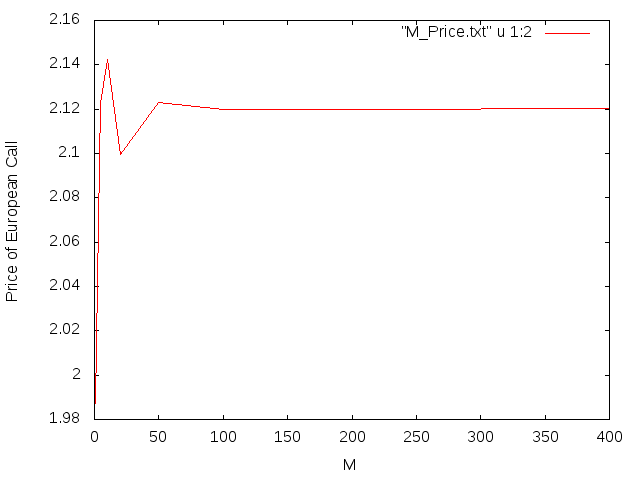
\includegraphics[width=80mm]{M_Price}
\end{center}

\begin{center}
M(increased in steps of 1) - Price of European call option Plot :\\
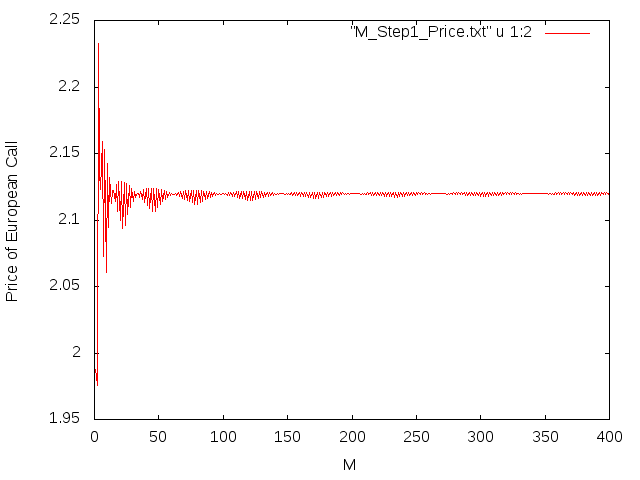
\includegraphics[width=80mm]{M_Step1_Price}
\end{center}

\begin{center}
M(increased in steps of 5) - Price of European call option Plot :\\
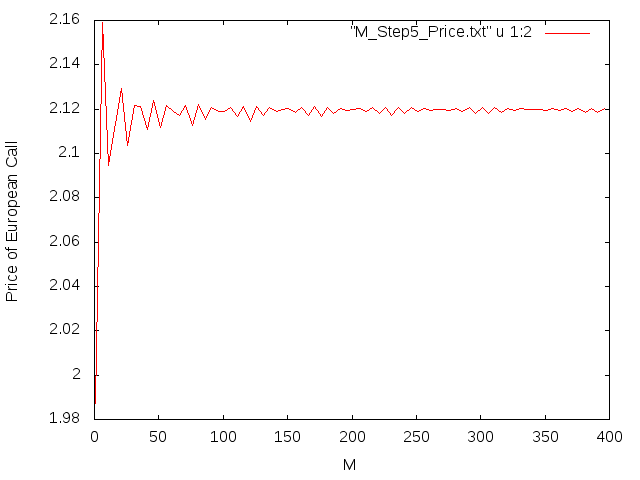
\includegraphics[width=80mm]{M_Step5_Price}
\end{center}

\newpage
European Put :
\begin{center}
M(Given in Part-1) - Price of European put option Plot :\\
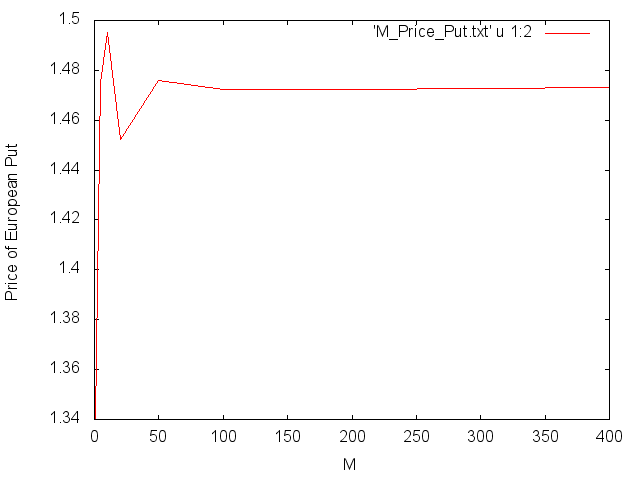
\includegraphics[width=80mm]{M_Price_Put}
\end{center}

\begin{center}
M(increased in steps of 1) - Price of European put option Plot :\\
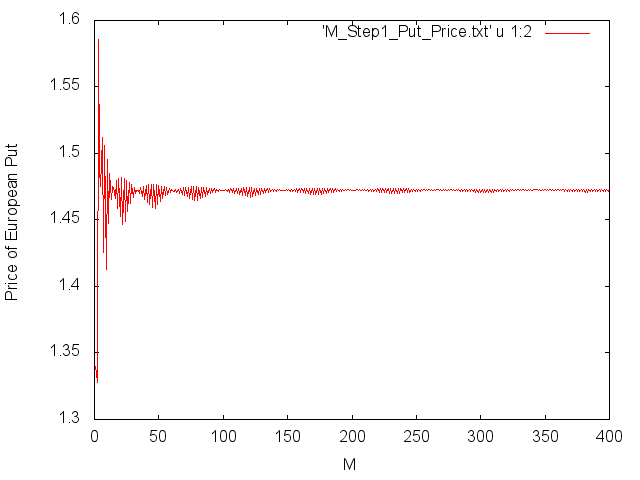
\includegraphics[width=80mm]{M_Step1_Put_Price}
\end{center}

\begin{center}
M(increased in steps of 5) - Price of European put option Plot :\\
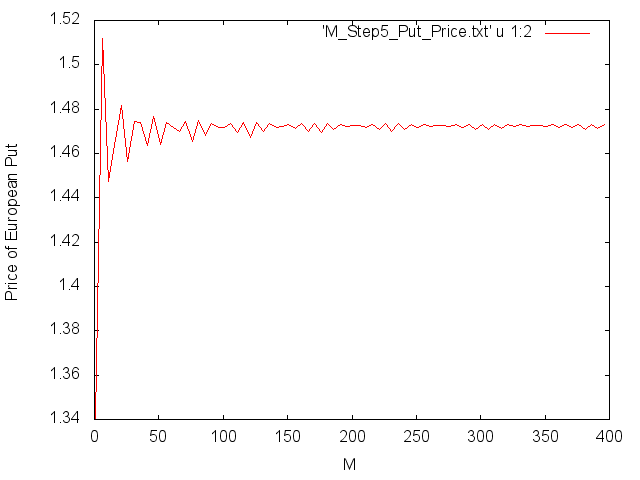
\includegraphics[width=80mm]{M_Step5_Put_Price}
\end{center}
Convergence in the price of option : As observed in the plot , the points of convergence are as follows :\\
(1) European Call Option :  M ( Step of 1 ) = 150(approx) ,  M ( Step of 5 ) = 200(approx) \\
(1) European Put Option :  M ( Step of 1 ) = 200(approx) ,  M ( Step of 5 ) = 200(approx) \\
\textbf{Part-3}\\
European Call :
\begin{center}
\begin{tabular}{ |c|c| } 
 \hline
 t & Value of Option \\
 \hline
2.70 & 56.296 , 42.586 , 31.719 , 23.106 , 16.278 , 10.866 , 6.576 , 3.176 , 0.892 , 0.054 , 0.000 \\
1.50 & 18.113 , 12.473 , 8.054 , 4.709 , 2.378 , 0.978 , 0.304 , 0.064 , 0.008 , 0.000  \\
0.75 & 7.151 , 4.237 , 2.241 , 1.024 , 0.389 , 0.118 \\
0.30 & 3.559 , 1.880 , 0.871 \\
0.00 & 2.100\\

 \hline
\end{tabular}
\end{center}

European Put :
\begin{center}
\begin{tabular}{ |c|c| } 
 \hline
 t & Value of Option \\
 \hline
2.70 & 0.000 , 0.411 , 1.709 , 3.349 , 4.691 , 5.755 , 6.598 , 7.266 , 7.796 , 8.216 , 8.549 , 8.813\\ 
1.50 & 0.001 , 0.011 , 0.071 , 0.277 , 0.760 , 1.591 , 2.685 , 3.846 , 4.901 , 5.774 , 6.471\\ 
0.75 & 0.227 , 0.560 , 1.139 , 1.962 , 2.944 , 3.955\\ 
0.30 & 0.831 , 1.481 , 2.319\\ 
0.00 & 1.452\\
 \hline
\end{tabular}
\end{center}

\end{document}